\subsection{Choice of the Penalty Weights}
The contributions \eqref{eqn:departure_delay_model_qubo_unique} and \eqref{eqn:departure_delay_model_qubo_conflict} to the QUBO for the departure delay model of section \ref{sec:departure_delay_model} are hard constraints.
This means a solution to the QUBO is only valid if both \eqref{eqn:departure_delay_model_qubo_unique} and \eqref{eqn:departure_delay_model_qubo_conflict} vanish.
Therefore, the penalty weights $\lambda_\text{unique}$ and $\lambda_\text{conflict}$ must be chosen sufficiently large to ensure that the hard constraints are fulfilled for the solution to the problem.
On the other hand, large penalty weights lead to large differences between the largest and smallest non-vanishing coefficients in the QUBO.
Since the D-Wave quantum annealers have a limited resolution for the specification of the QUBO, this can lead to a misspecification of the problem. \footnote{Reference to D-Wave limited resolution}
Hence, it is desirable to find a sweet spot of the smallest penalty weights which still yield valid solutions.

\begin{figure}[htpb]
    \centering
    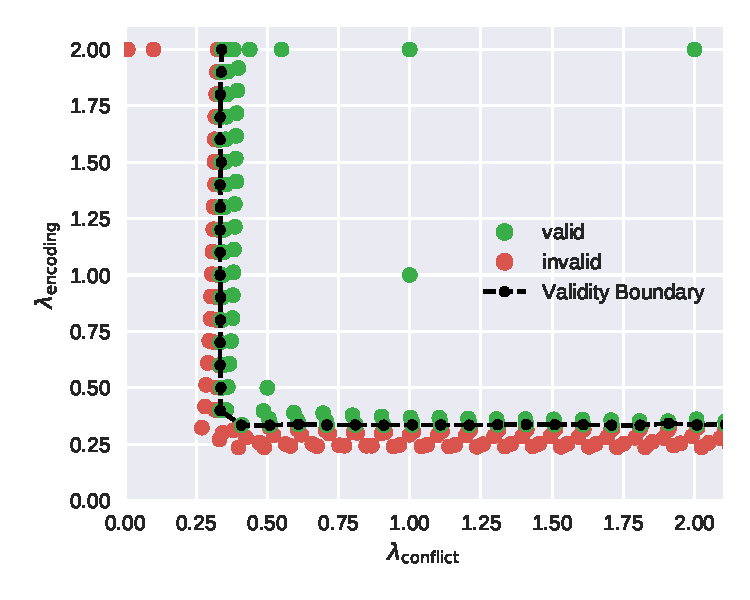
\includegraphics[width=0.45\textwidth,natwidth=1,natheight=0]{./pics/validity_boundary_example.pdf}
    \caption{Validity of exact solution to a QUBO extracted from a problem instance with $N_f=7$ flights and $N_c=9$ conflicts in dependence on the choice of the penalty weights, $\lambda_\text{unique}$ and $\lambda_\text{conflict}$. Here, $\Delta_t=3$ and $d_\text{max}=18$.}
    \label{fig:penalty_weights}
\end{figure}

In order to find these optimal penalty weights, we employed an exact solver \footnote{Reference to mapping from QUBO to max sat and to akmaxsat solver} to explore the validity of a solution in dependence on the penalty weights.
We investigated problem instances with up to $N_f=7$ flights and $N_c=9$ conflicts.
For all these problem instances we found a box like shape of the boundary between valid and invalid solutions as it is depicted in figure \ref{fig:penalty_weights}.

One can give an upper bound for the sufficiently large penalty weights by the following considerations.
A minimal violation of the hard constraints yield an additional contribution to the QUBO cost function of $\lambda_\text{unique}$ or $\lambda_\text{conflict}$, respectively.
Such a violation would correspond to single bit flip in the binary delay variables $d_{i\alpha}$.
Therefore the contribution from \eqref{eqn:departure_delay_model_qubo_departure} would be reduced maximally by 
\begin{equation*}
    \min_\alpha \frac{-\alpha}{d_\text{max}} = - 1    
\end{equation*}
Hence, sufficiently large penalty weights must fulfill the following conditions
\begin{align*}
    \lambda_\text{unique} & > 1 \\
    \lambda_\text{conflict} &> 1 \, .
\end{align*}
This corresponds to a box like shape as it appears in figure \ref{fig:penalty_weights}.
